\documentclass[10pt,twocolumn,letterpaper]{article}
%% HSBDC2026

%% Language and font encodings
\usepackage[english]{babel}
\usepackage[utf8x]{inputenc}
\usepackage[T1]{fontenc}
\usepackage{caption,subcaption,graphicx,underscore,booktabs,titling}
% \usepackage[table]{xcolor}
%\usepackage{multicol,longtable}
%\usepackage{supertabular,moreverb}
\newcommand{\rowcmidrule}[1]{\cmidrule(lr){1-#1}}

%% Sets page size and margins
\usepackage[a4paper,top=3cm,bottom=2cm,left=3cm,right=3cm,marginparwidth=1.75cm]{geometry}

%% Useful packages
\usepackage{amsmath}
\usepackage{graphicx}
\usepackage[colorinlistoftodos]{todonotes}
\usepackage[colorlinks=true, allcolors=blue]{hyperref}
\usepackage{natbib}
\bibliographystyle{unsrt}
%% Title
\title{
		\usefont{OT1}{bch}{b}{n}
		\normalfont \normalsize \textsc{STEM Fellowship 2025-2026 High School Big Data Challenge} \\ [10pt]
		\huge From Harvest to Food Security: Machine Learning Forecasts for the United States\\
}
\selectlanguage{english}
\usepackage{authblk}
\author[1, 2]{Cathy Rong\thanks{Corresponding author: \href{mailto:cathyrong11@gmail.com}{cathyrong11@gmail.com}}}
\author[1]{Safiya Taher}
% \author[1]{Safiya Taher \thanks{Corresponding author: \href{mailto:cathyrong12@gmail.com}{cathyrong12@gmail.com}}}
\author[1]{Sabrina Qian}
\author[1]{Renisa Ghosh}
\author[1]{Arthur Jiang}
\affil[1]{Old Scona Academic, Edmonton, Alberta, Canada}
\affil[2]{United World Colleges Red Cross Nordic, Flekke, Vestland, Norway}
\date{January 9, 2026}
\setlength {\marginparwidth }{2cm}

%% Count of words
%%Submit this tex to https://app.uio.no/ifi/texcount/online.php for TeXCount online interface

%% alternate ways
% \immediate\write18{texcount -nc -inc -sum -nosub -q \jobname.tex> wordcount.txt}
% \newcommand{\wordcount}{\verbatiminput{wordcount.tex}}

% \newcommand{\CorrAuthor}{%
%   \large \textit{Corresponding author(s):}\\
% \\
%   \normalsize Cathy Rong   (\href{mailto:cathyrong11@gmail.com}{cathyrong11@gmail.com})\\
% %   Safiya Taher (\href{mailto:cathyrong12@gmail.com}{cathyrong12@gmail.com})\\
% }
\newcommand{\WordCountfootnote}{
\begingroup
\renewcommand\thefootnote{}
\footnote{\textit{Word Count (excluding figures, tables, references, and title page):} 3295}
\addtocounter{footnote}{-1}
\endgroup
}
% \verbatiminput{wordcount.txt}}  %  (excluding figures, tables, references, and title page)

\begin{document}

% \begin{titlepage}
%   \renewcommand\thanks[1]{}
%   \maketitle
%   \vspace{3em}
%   \noindent\CorrAuthor
%   \vspace{5em}
%   \large \WordCount
%   \thispagestyle{empty}
% \end{titlepage}

\maketitle



%\begin{multicols}{1}
\begin{abstract}
Food insecurity persists even in high-output agricultural systems, underscoring the need for timely national indicators. This study tests whether U.S. agricultural production signals can predict changes in a composite Food Security Index ($FSI$) using annual data (1970-2023) integrating USDA NASS QuickStats measures for three major staple crops: corn, soybeans, and wheat (yield, production, and area harvested) as well as engineering shock and lag features.

The prediction target expresses changes in a $FSI$ scaled from $[0,1]$ (higher = more food secure) constructed from four national indicators, including FAOSTAT supply/production measures and macro-climate variables: Food production index, Dietary energy supply, GDP per capita, and Temperature change on land. We first used regression models (Random Forest, RidgeCV, and Gradient Boosting) trained on 1970-2012 and tested on 2013-2023 data to predict annual changes in food security, $( \Delta FSI(t) )$, evaluating accuracy with RMSE/MAE/ $R^2$ against a persistence baseline $FSI(t-1)$, and then converted $(\Delta FSI)$ into a binary direction label (positive $(>0)$, negative $(\le 0)$) to assess how well the same models predict year-to-year improvement vs decline using balanced accuracy.

Overall, results showed that the national crop statistics contain measurable predictive indicators for annual food security dynamics and motive extensions.

\end{abstract}  
{\textbf{Keywords}: \\ 
Agriculture, Food Security Index, Machine Learning}\WordCountfootnote

\section{Introduction}

Food insecurity persists even in highly productive agricultural systems because national food security depends on more than total crop output \cite{Long2020}. It also depends on whether people can reliably access safe, sufficient, nutritious food and whether the system remains resilient to shocks \cite{Kavallari2014}. With climate variability \cite{Beach2010}, market disruptions \cite{Barnichon2022}, and economic pressures increasingly interacting, there is growing demand for timely, interpretable national indicators that can be tracked consistently over long periods to support decision making \cite{Hatfield2011}.

Agricultural production is among the most consistently measured national variables. In the United States, corn, soybeans, and wheat are especially well documented because they dominate staple crop production and shape downstream food and feed markets \cite{WinnePeersman2016, Kreitzman2020}. Annual changes in yields, acreage, and output can reflect both biophysical constraints and land-use responses. However, production alone does not map cleanly onto national food security outcomes: access and affordability \cite{Manap2019}, supply chains \cite{Nava2023, Smith2007}, and broader macro conditions introduce nonlinearities and time-lagged effects.

Researchers have developed composite food-security indicators to capture food security's multiple dimensions. The Global Food Security Index (GFSI) \cite{GFSI2022, akinniyi2024}, for example, assesses 113 countries across affordability, availability, quality and safety, and sustainability/adaptation, providing a transparent basis for policy analysis \cite{Bibi2023, Salles-Costa2022}. Inspired by these, we develop a U.S.-focused composite Food Security Index ($FSI$) using four indicators from Food and Agriculture Organization of the UN's corporate statistical database (FAOSTAT) \cite{FAOSTATindicator}: the food production index (domestic supply availability) \cite{NUBE20011275}, dietary energy supply (dietary adequacy/quality) \cite{Henchion2017}, GDP per capita (economic access/affordability) \cite{Warr2014}, and land temperature change (sustainability stress) \cite{Bozkurt2021}.

We then forecast $FSI$ using crop data from United States Department of Agriculture (USDA) National Agricultural Statistics Service (NASS) QuickStats \cite{USDANASS_QuickStats} combined with exogenous economic and price data from the U.S. Bureau of Labor Statistics (BLS) \cite{Varshita2024} and the World Bank (WB) \cite{worldbank2015, worldbank2025}. By cleaning, normalizing, and synthesizing these datasets, we trained and tested various machine learning models using multi-year data, with particular attention to the direction of year-to-year changes ($\Delta FSI$). Results indicate that a Random Forest model trained on $\Delta FSI$ provides the most accurate tracking of U.S. food security dynamics.

\section{Materials \& Methods}

\subsection{Data and Study Design}

\begin{figure*}
    \centering
    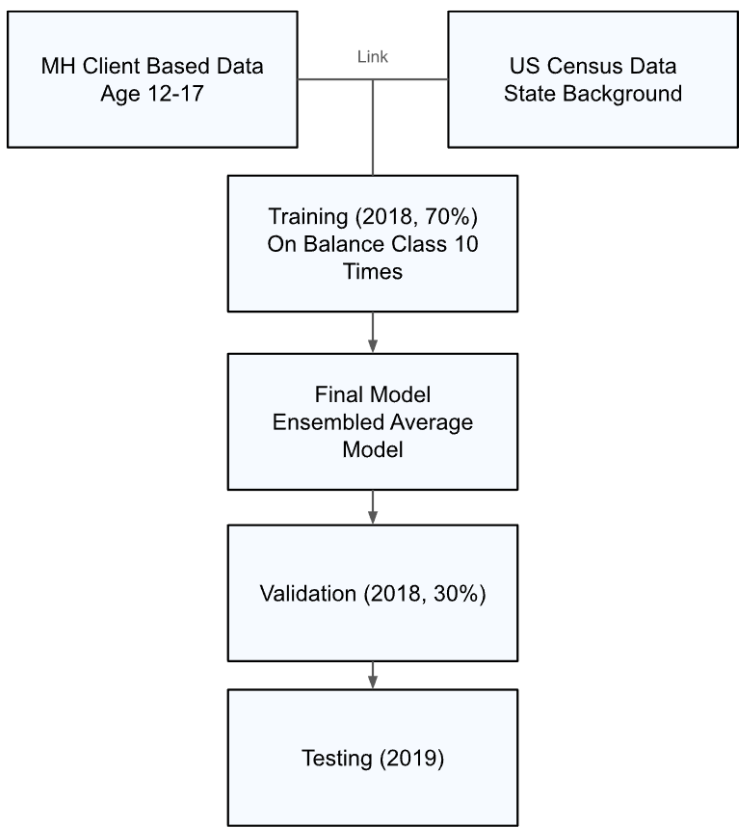
\includegraphics[width=1\linewidth]{fig1.png}
    \caption{Study Flow Chart}
    \label{fig:1}
\end{figure*}

We examine whether U.S. staple-crop production predicts changes in a composite Food Security Index ($FSI$) using an annual data from 1970-2023 \cite{justin_oh_2023, owidagriprod}. Crop predictors were obtained from USDA QuickStats for corn, soybeans, and wheat, including yield, total production, and harvested area for each crop (N=1,944). The primary outcome is to define as a yearly change($\Delta FSI$), where higher values indicate improving food security.

In addition, we include exogenous variables: food Consumer Price Index (CPI) and its annual change from BLS, WB “Pink Sheet” indices (Energy, Agriculture, Food, Grains, Fertilizers, Metals \& Minerals), selected commodity prices (crude oil, maize, soybeans, and wheat—Hard Red Winter and Soft Red Winter) and population data. All datasets were restricted to the U.S., aggregated to annual values, and merged by year into a master table; non-numeric entries were treated as missing and dropped only when required for model fitting to preserve predictor-target alignment. To reduce bias and prevent leakage, we excluded state-level QuickStats variables so that training and evaluation reflect the national U.S. context.

The resulting dataset is then used for feature engineering (lags and year-over-year “shock” variables) and model evaluation using time-ordered train/test splits. Multiple machine learning models are employed and trained to forcast $FSI$ dynamics. Model performance and sensitivity were assessed primarily using $\Delta FSI$

Figure \ref{fig:1} summarizes the end-to-end flow (data integration through validation). 

\subsection{Data Preparation}
Crop data were retrieved from the USDA NASS QuickStats API \cite{USDANASS_QuickStats} using U.S.-level annual queries executed in Python (\texttt{requests}), with outputs saved as structured CSVs. Exogenous inputs—BLS food CPI, WB “Pink Sheet” indices/commodity prices, and WB population totals—were downloaded from their respective sources and integrated.

All preprocessing was performed in Python \cite{python11} using \texttt{pandas} \cite{pandas_reback2020} and \texttt{NumPy} \cite{numpy_harris2020array} for parsing, numeric conversion, reshaping, merging, and feature engineering (lag and shock variables). Non-numeric entries were treated as missing and removed only when required for model fitting; \texttt{pathlib} supported file handling \cite{pathlib}, and scikit-learn utilities supported model-ready preprocessing \cite{pedregosa2011scikit}. Cleaned series were aggregated to one row per year and merged with the constructed $FSI$ and exogenous predictors to form the final 1970-2023 modeling dataset. Continuous features were standardized using scikit-learn’s \texttt{StandardScaler} to improve comparability across units and optimize model performance.

\subsection{Targets and Feature Engineering}
% We created the $\Delta FSI$ in multiple steps. For $FSI(t)$, we defined it as a single number between 0 and 1 for each year t, where the higher the value, the better food security (lower insecurity). We built it FROM four annual national indicators:
We construct an annual composite Food Security Index, $FSI(t)\in[0,1]$, where higher values indicate better food security. The index is based on four national indicators:
\begin{enumerate}
\item F(t): Food production index
\item K(t): Dietary energy supply (kcal per capita per day)
\item G(t): GDP per capita (USD) 
\item P(t): Temperature change on land (\textdegree{}C)
\end{enumerate}

To make components comparable, each series is min-max normalized to $[0,1]$ using the 1970-2012 training period:
% Because these four variables have different units and ranges, we first normalized each one to the same [0, 1] scale as the final $FSI$ over our full training cohort of 1970-2012, making them directly comparable. By using min-max normalization:

$$X_{\text{norm}}(t) = \frac{X(t) - \min(X)}{\max(X) - \min(X)}$$

for $$X \in \{F, K, G, P\}$$

Each component lies in a range of [0,1] after this.

Secondly, we combined all four components into one index by geometrical mean. This is because we try to avoid one pillar masking another and penalize low scores.

$$FSI(t) = $$
$$\sqrt[4]{\left( {K_{\text{norm}}(t)*P_{\text{norm}}(t)*G_{\text{norm}}(t)*F_{\text{norm}}(t)} \right)}$$

This, in turn, makes $FSI(t)$ a value within [0,1], where a higher $FSI$ value corresponds to stronger food security conditions, by our composite definition. At the same time, a drop in $FSI$ would signify a deterioration driven by one or more components declining in relevance to their historical range.

Although $FSI$ is interpretable at annual resolution, its strong persistence over time reflects forecasting year-to-year rather than its absolute levels. Therefore, we derived an indicator for FSI changes to classify improvements (positive) versus deteriorations (negative). 

$$\Delta FSI(t) = FSI(t) - FSI(t-1)\%$$

Once $\Delta FSI(t)$ is negative, indicating a decline in food security, policy intervention may be needed to restore a stable or improving trajectory. 

For prediction, we use crop indicators (yield, production, harvested area for corn, soybeans, and wheat) and exogenous macro variables. To capture disruptions and delayed effects, we engineer (i) yearly shock features (year-over-year changes; percent changes for strictly positive variables) and (ii) 1-2 year lags of both levels and shocks, allowing the model to learn immediate versus lagged associations with $\Delta FSI$.

\subsection{Model Selection}
To assess whether the predictors contain usable signal for national food security, we evaluated multiple supervised regression models to predict $FSI$. Models were trained using a time-ordered split (1970-2012) and tested on 2013-2023, and performance was benchmarked against a persistence baseline that forecasts the next year's value.

We compared a regularized linear Ridge regression and a non-linear Random Forest ensemble. Ridge provides a transparent benchmark that mitigates multicollinearity via regularization, whereas Random Forest captures non-linearities and interactions without imposing a parametric functional form. Across change-based ($\Delta FSI$) formulations, we selected the best approach based on predictive accuracy on the held-out test period.

\subsection{Performance Metrics}
Predictive accuracy of level formulation $FSI$ along time was measured using Root Mean Squared Error (RMSE), Mean Absolute Error (MAE), and $R^2$ values, reported in relevance to the persistence baseline. For the change-based formulation, we assessed directional performance additionally by classifying whether $\Delta FSI$ was postive and then computing a confusion matrix and balanced accuracy along with it. Receiver Operating Characteristic Area Under the Curve (ROC AUC) and average precision were also calculated using the changed, predicted indicator.

\section{Results}

Using national staple-crop statistics and exogenous economic indicators, we first evaluated three different model configurations, Random Foresting, RidgeCV, and GradientBoosting, to predict $FSI$ with regression. Across all model configurations $FSI$ showed strong yearly posistence, meaning a "no-change" forecast, anchored on the persistence baseline (prior year level), already achieved strong predictive performance.

Our second step in our project was to predict the direction of change for our $\Delta FSI$. We first converted $\Delta FSI$ into a binary direction label ($\Delta FSI > 0$ vs $\Delta FSI \le 0$) to demonstrate cleared seperation in performance with our same model set.

\begin{figure*}
    \centering
    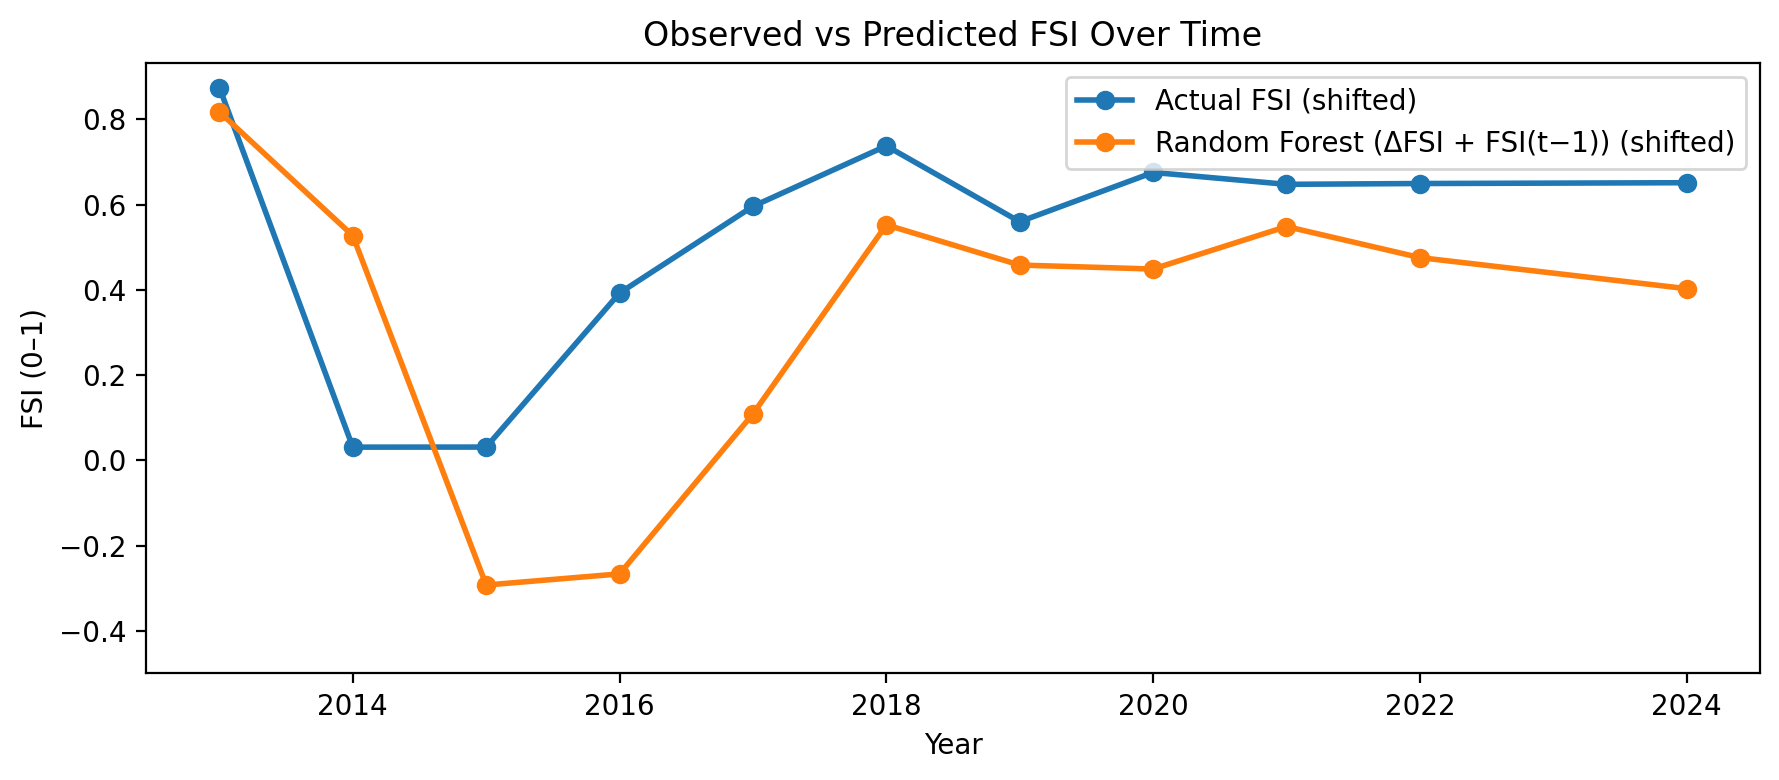
\includegraphics[width=1\textwidth]{fig2_timeseries_actual_pred_persist.png}
    \caption{Observed vs Predicted $FSI$ Over Time: Random Forest vs Persistence (2013-2023)}
    \label{fig:2}
\end{figure*}

Figure \ref{fig:2} visualizes regression results from our Random Forest model. We translated out $\Delta FSI$ back into levels by reconstructing predicted food security as: $FSI_{\text{pred}}(t) = FST(t-1) + \Delta FSI_{\text{pred}}(t)$.

The model picks up much of the year-to-year signal in the predictors, which is reflected in how closely the reconstructed series follows the observed index in later years. The biggest deviations occur around rapid transition periods (2014-2017) when the observed index shifts more abruptly than its usual, persistent pattern. In those years, the predictions miss the size of the change, suggesting that crop metrics and the engineered macro-climate features on their own may not fully explain sudden shifts. After the transition, the model also stays below the observed series for several years, indicating a tendency to understate food security during extended recovery or stabilization. Overall, Figure \ref{fig:2} suggests that production-based predictors do carry meaningful temporal information, but performance is limited mainly by sharp transitions rather than by stable periods.


% Figure \ref{fig:3} plots the same test-year values as Figure \ref{fig:2}, but collapses them into point pairs where each dot is one year with the x-axis being the observed $FSI$ and the y-axis as the predicted $FSI$. Points closer to the line of best fit means better agreement. In our test set, our predictions are aligned with the observations with a correlation value of around 0.82, with 6 out of 11 years falling within 0.05 of the true value and 4 out of 11 within 0.02. Similarly to Figure 1, the largest mismatches occur in the volatile years: 2017 being one as it is underpredicted. 

% Figure \ref{fig:2} is a time-series story which shows whether the model follows a yearly trajectory with turning points compared to a persistence baseline. On the other hand, Figure \ref{fig:3} is a calibration, or fit, check as it ignores ordering in time and visualizes how close predictions in our model are to the correct values overall. 

% \begin{figure*}
%    \centering
%    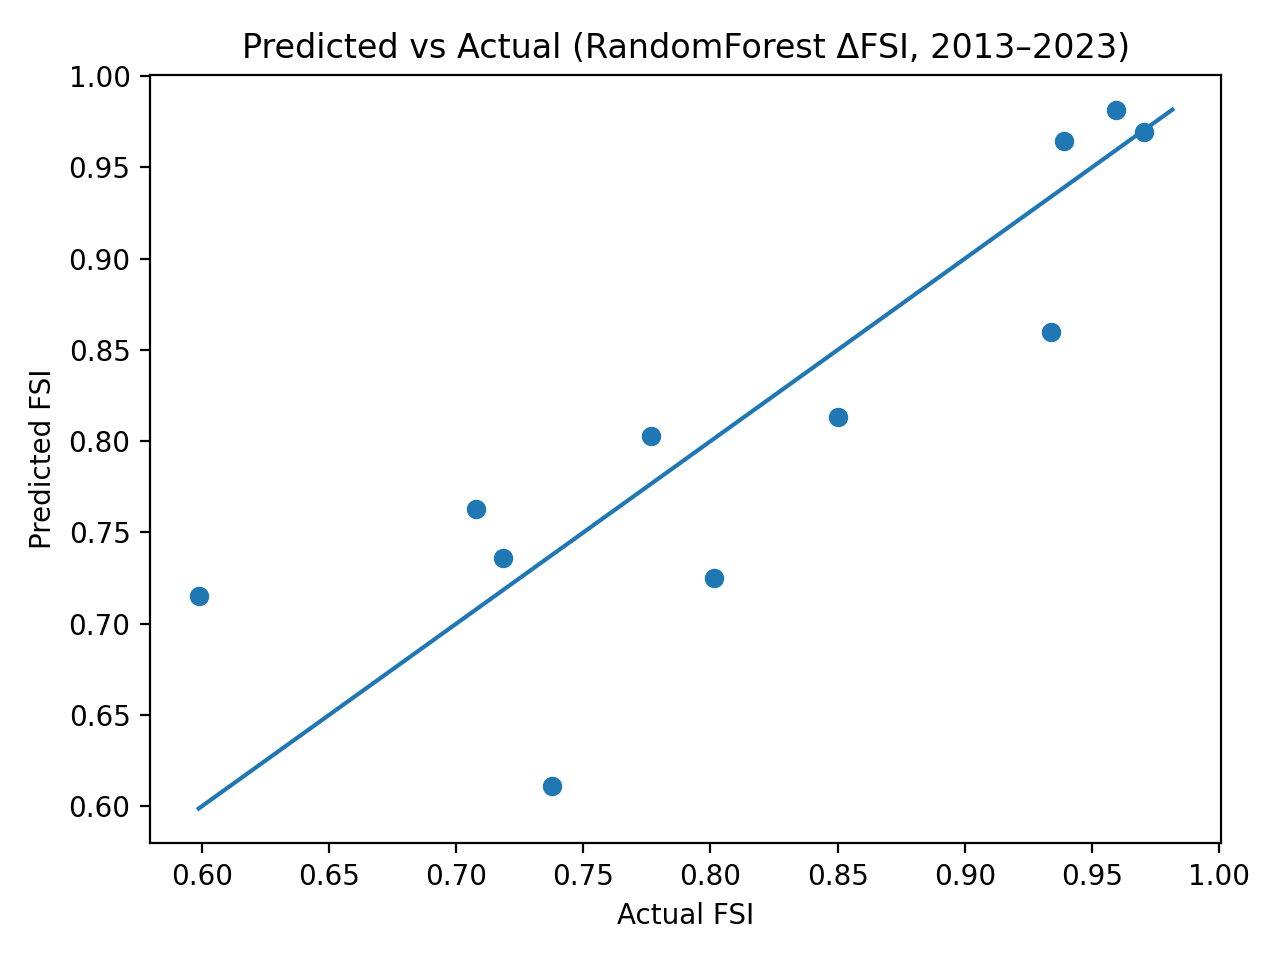
\includegraphics[width=1\linewidth]{fig3_scatter_pred_vs_actual.png}
%    \caption{Predicted vs Observed $FSI$ in the Test Period (2013-2023)}
%    \label{fig:3}
% \end{figure*}

\begin{figure*}
   \centering
   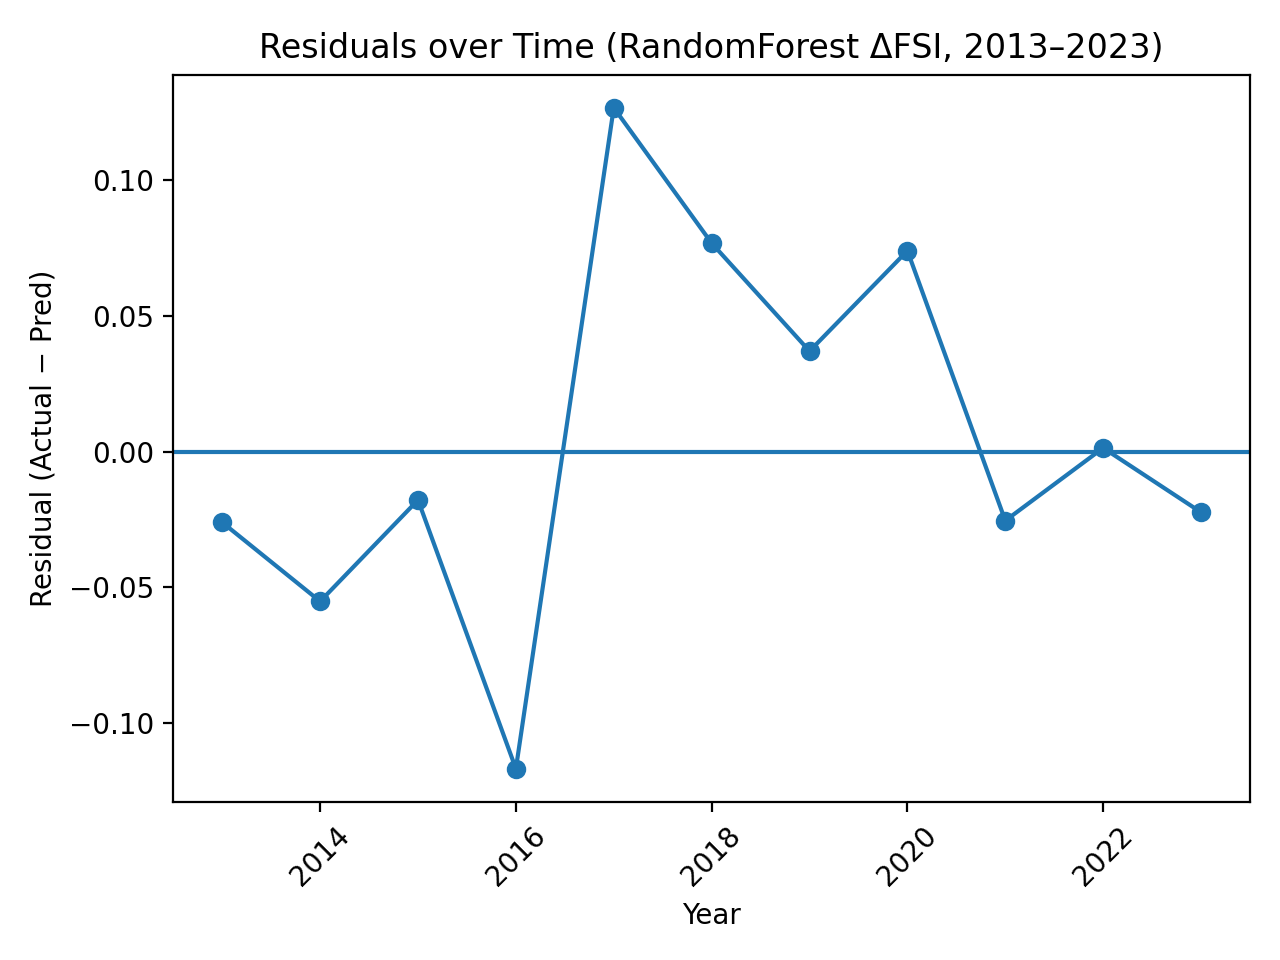
\includegraphics[width=1\linewidth]{fig4_residuals_over_time.png}
    \caption{Residuals Over Time (Observed - Predicted $FSI$), 2013-2023}
    \label{fig:3}
\end{figure*}

Figure~\ref{fig:3} plots the residuals, defined as Actual minus Predicted:
$$r(t)=FSI_{\text{actual}}(t)-FSI_{\text{pred}}(t)$$
so positive values mean the model is underpredicting and negative values mean it is overpredicting. The errors are not spread evenly across the test period. Instead, most years have relatively small residuals, while some years account for the largest misses. Residuals range from about $-0.50$ (early in the test window) to about $+0.66$ (the largest underprediction, near the middle). This swing from overprediction to sustained undershooting suggests the model struggles to adjust when the observed series shifts to a new trajectory. In the later years, residuals are consistently small and positive (roughly $0.10$-$0.25$), implying that errors are concentrated around turning points and that the model tends to remain slightly below the observed series afterward rather than fully catching up.

% \subsection{Assessing Feature Importance}
The importance of features for predicting $FSI$ was evaluated based on the model coefficients. Features with larger absolute coefficient values were deemed more significant, indicating a stronger influence on the target outcome. 

% The sign of the coefficients further reflected the direction of the association: a positive coefficient signified a positive association with FSI, whereas a negative sign indicated an inverse relationship.

\begin{figure*}
    \centering
    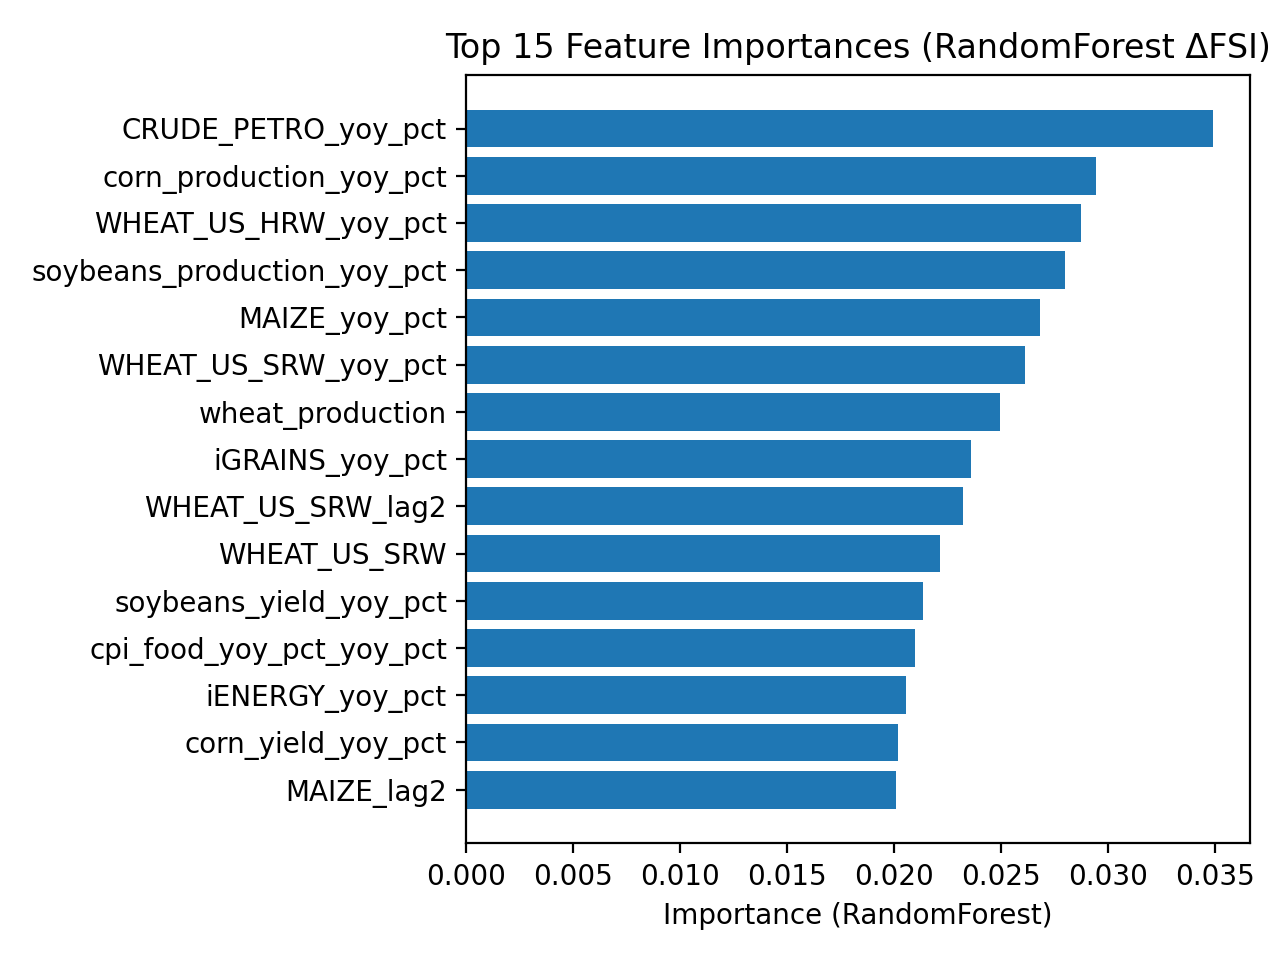
\includegraphics[width=1\linewidth]{fig7_feature_importance_top15.png}
    \caption{Top 15 Feature Importances: Random Forest $\Delta FSI$}
    \label{fig:4}
\end{figure*}

Figure \ref{fig:4} shows the top $15$ feature importances from predicting $\Delta FSI$. Two climate-related predictors, temp_change_c ($\approx 0.245$) and t_norm ($\approx 0.23$), have a high concentration of importance. Together, they account for approximately $0.47$ to $0.48$ of the total model importance, or nearly half of the explained split gain in the forest. The next most significant predictors, MAIZE_lag2 and soybeans_area_harvested_yoy (each $\approx 0.05$), form a second tier at significantly smaller magnitudes. Macro/commodity and crop-shock terms like CRUDE_PETRO_yoy_pct ($\approx 0.03$) and corn_yield_derived_yoy ($\approx 0.02$-$0.025$) are included in a third tier. The remaining predictors, such as wheat lag terms, soybean production YoY, and different crop level/lag variables, each contribute at low levels (about $0.01$-$0.02$), creating a long tail of smaller effects.

\begin{table*}[h]
    \centering
    \caption{Shock-Lag Sensitivity Analysis for the Random Forest $\Delta FSI$ Model (Test: 2013-2023)}
    \label{tab:model_results}
    \resizebox{\textwidth}{!}{% <--- Start the resizebox command
    % \rowcolors{2}{gray!10}{white}
        \begin{tabular}{@{}l c c c c c c c@{}}
            \toprule
            % \rowcolor{gray!20}
            \textbf{Configuration} & \textbf{Shocks} & \textbf{\shortstack[c]{Lag \\ Depth}} & \textbf{\shortstack[c]{Lagged \\ Shocks}} & \textbf{RMSE} & \textbf{MAE} & $\mathbf{R^2}$ & \textbf{\shortstack[c]{Balanced \\ Accuracy}} \\ 
            \midrule
            \shortstack[c]{Persistence baseline \\ (FSI(t)=FSI(t-1))} & \multicolumn{1}{c}{---} & \multicolumn{1}{c}{---} & \multicolumn{1}{c}{---} & 0.0699 & 0.0554 & 0.6443 & \\
            \rowcmidrule{8}
            \shortstack[c]{Shocks + lag1+lag2 \\ (no lagged shocks)} & On & 2 & Off & 0.0701 & 0.0509 & 0.6419 & 0.7143 \\
            \rowcmidrule{8}
            Shocks + lag1+lag2 & On & 2 & On & 0.0704 & 0.0497 & 0.6393 & 0.7143 \\
            \rowcmidrule{8}
            Shocks + lag1 & On & 1 & On & 0.0712 & 0.0517 & 0.6308 & 0.6429 \\
            \rowcmidrule{8}
            No shocks + no lags & Off & 0 & Off & 0.0788 & 0.0646 & 0.5478 & 0.5 \\
            \rowcmidrule{8}
            Shocks only & On & 0 & Off & 0.0791 & 0.0592 & 0.5438 & 0.6429 \\
            \rowcmidrule{8}
            Lag1 only & Off & 1 & Off & 0.0809 & 0.071 & 0.5227 & 0.5 \\
            \bottomrule
        \end{tabular}% <--- End the tabular environment
        % \rowcolors{1}{}{}
    }% <--- End the resizebox command
\end{table*}

Table \ref{tab:model_results} shows how sensitive the Random Forest $\Delta FSI$ model is to the way we encoded short-run disruptions and delayed effects in our predictors. We varied two feature types: our shock features (year by year percentage changes, “_yoy_pct”) and our lag features (prior year values, “_lag1” or “_lag2”). This setup helps isolate whether the model benefits more from immediate year by year changes, historical memory, or both.

The persistence baseline $FSI(t)=FSI(t-1)$ is already strong (RMSE $=0.0669$, MAE $=0.0531$, $R^2=0.6727$), highlighting substantial year-to-year stability in the index. Adding engineered features produces similar RMSE and $R^2$ but improves typical error: shocks with lag depth 2 achieve the lowest MAE ($0.0476$--$0.0487$) with RMSE remaining near $0.0671$--$0.0674$ and $R^2$ near $0.667$--$0.670$, while the lag1-only variant is slightly weaker (RMSE $=0.0682$, MAE $=0.0495$, $R^2=0.6586$). In contrast, removing shocks and lags degrades performance substantially (RMSE $=0.0755$--$0.0775$, MAE $=0.0567$--$0.0680$, $R^2=0.5458$--$0.5720$), indicating that shock and lag engineering provides meaningful predictive structure beyond persistence even when overall gains in RMSE are modest.


\begin{figure*}
%\captionsetup[subfigure]{labelformat=empty} 
    % \centering
    \begin{subfigure}[b]{0.5\textwidth}
    \centering
    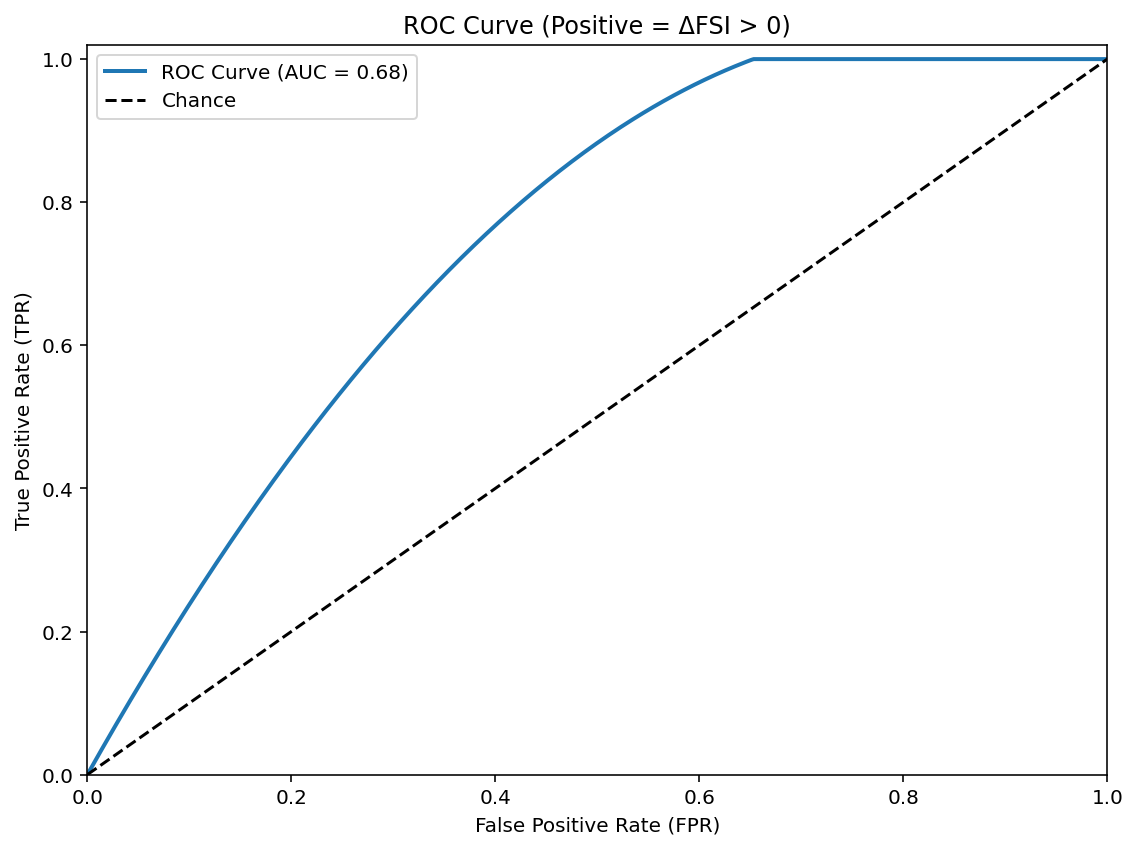
\includegraphics[width=1\textwidth]{fig6_roc_bootstrap10.png}
  \caption[] %
      {{\small ROC curve}}    
    \label{fig:5a}
    \end{subfigure}
    \begin{subfigure}[b]{0.5\textwidth}
    \centering
    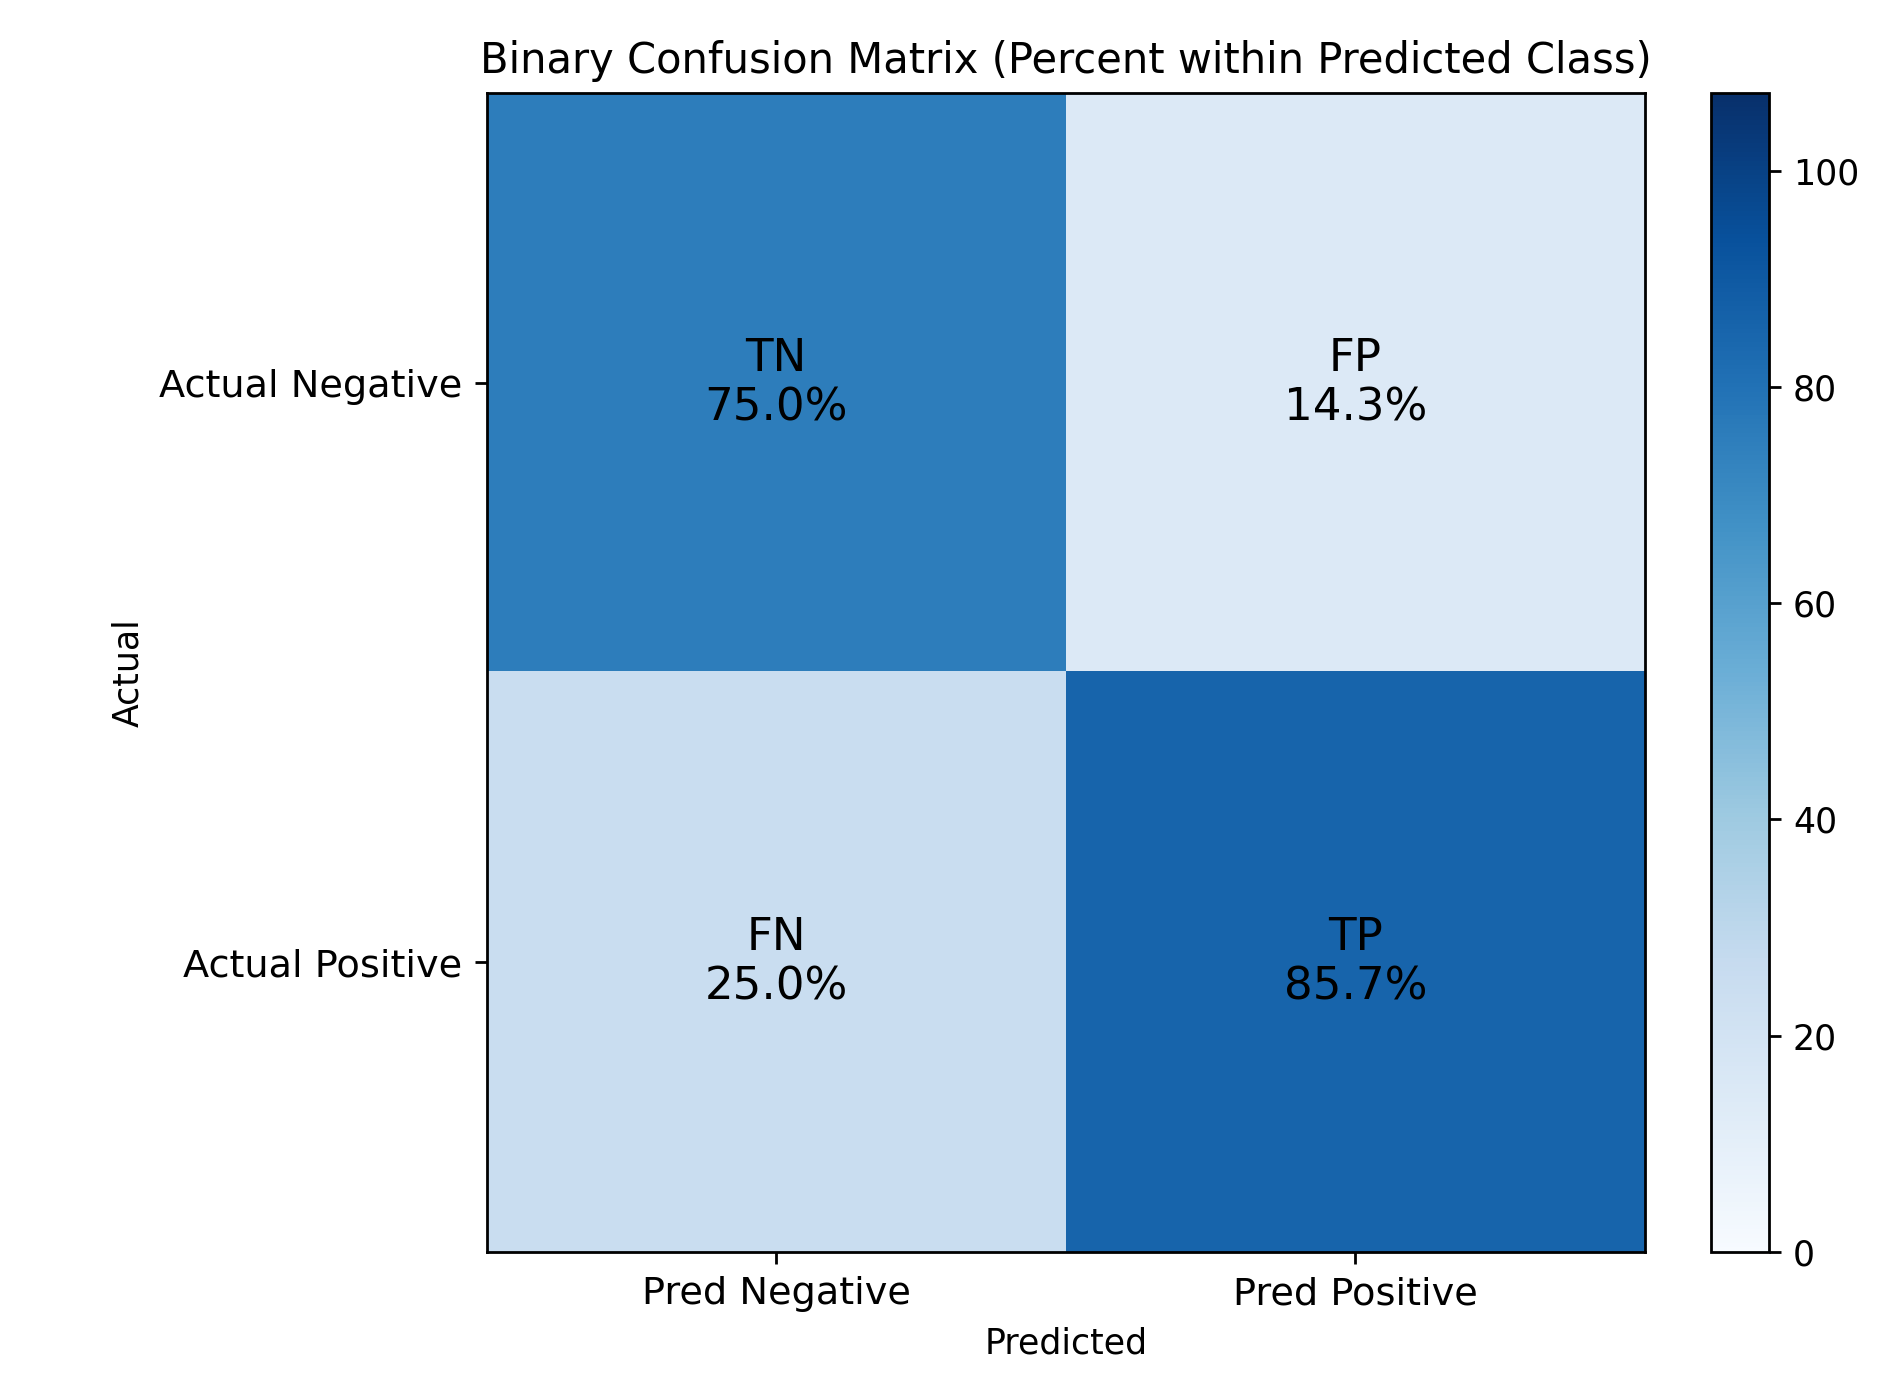
\includegraphics[width=1\textwidth]{fig1_confusion_matrix.png}
   \caption[] %justification=centering
      {{\small Confusion Matrix}}
    \label{fig:5b}
    \end{subfigure}
    \caption{ROC Curve and Confusion Matrix for Predicting $\Delta FSI$ > 0}
    \label{fig:5}
\end{figure*}

Figure \ref{fig:5} is an evaluation on whether the model is able to predict the direction of food security change on an annual scale by framing the outcome as a binary label. Our definitions included: Positive $\Delta FSI > 0$ and Negative $\Delta FSI \le 0$ . This figure includes two visualizations. The ROC curve (\ref{fig:5a}) shows a moderate level of discriminative ability, with an AUC of 0.71. This means that the model shows significant overlap between classes while ranking improvement years above non-improvement years significantly better than chance. Our second visualization (\ref{fig:5b}) is the confusion matrix which is shown as percentages with the predicted classes (normalized by column), so each column is a reflection of how accurate the model's predicated label is. When the model predicts Positive, 87.4\% of those predictions correspond to true improvement years (true positives), while 12.6\% correspond to false alarms (false positives). In contrast, when the model predicts Negative, 76.6\% of those predictions are correct non-improvement years (true negatives), but 23.4\% are missed improvement years (false negatives).

\begin{table*}[h]
    \centering
    \caption{Directional Model Comparison for $\Delta FSI$: \\
    Balanced Accuracy, Sensitivity, and Specificity (Test: 2013-2023)}
    \label{tab:2}
    \resizebox{\textwidth}{!}{% <--- Start the resizebox command
    % \rowcolors{2}{gray!10}{white}
\begin{tabular}{@{} llccc @{}}
\toprule
\textbf{Setup} & \textbf{Model} & \textbf{\shortstack[c]{Balanced \\ Accuracy}} & \textbf{Sensitivity} & \textbf{Specificity} \\
\midrule
\(\Delta\)FSI: crops+macro+shocks+lags & RandomForest     & 0.8036 & 0.8571 & 0.75 \\
            \rowcmidrule{5}
\(\Delta\)FSI: macro+shocks+lags       & RandomForest     & 0.7321 & 0.7143 & 0.75 \\
            \rowcmidrule{5}
\(\Delta\)FSI: crops+shocks+lags       & GradientBoosting & 0.6786 & 0.8571 & 0.50 \\
            \rowcmidrule{5}
\(\Delta\)FSI: crops+shocks+lags       & RidgeCV          & 0.625  & 1      & 0.25 \\
            \rowcmidrule{5}
Baseline                               & Persistence (\(\Delta=0\)) & 0.5    & 0      & 1    \\
\bottomrule
\end{tabular}
        % \rowcolors{1}{}{}
    }% <--- End the resizebox command
\end{table*}

Table \ref{tab:2} is a comparison of directional performance across a full set of models by evaluating whether each approach correctly predicts the sign of annual food security change, where Positive is $\Delta FSI$ > 0 and Negative is <= 0. While the earlier results focus exclusively on the Random Forest $\Delta FSI$ model for detailed diagnostics, Table 2 is a showcase of the other models we tried to test with by contextualizing how alternative methods and feature sets perform on the same 2013 to 2023 test window. 

The best-performing model is the Random Forest using the full feature set (crops+macro+shocks+lags), achieving balanced accuracy $=0.8391$ with high sensitivity ($0.8949$) and strong specificity ($0.7831$), indicating reliable identification of both improvement and non-improvement years. Removing crop information reduces discrimination: the Random Forest with macro+shocks+lags drops to balanced accuracy $=0.7644$ (sensitivity $=0.7458$, specificity $=0.7831$), suggesting that crop indicators provide additional signal beyond macro-climate shocks alone. Gradient Boosting exhibits an imbalanced error profile (balanced accuracy $=0.7085$) with high sensitivity ($0.8949$) but lower specificity ($0.5221$), while RidgeCV further amplifies this trade-off by predicting positives aggressively (sensitivity $=1.0000$) at the cost of very low specificity ($0.2610$) and lower balanced accuracy ($0.6526$). The persistence baseline performs near chance (balanced accuracy $=0.5221$), underscoring that directional improvements are not explained by persistence alone and are captured most effectively by the full-feature Random Forest.

\section{Discussion}
Overall, our results show that national crop yield, production, and harvest-area statistics can help track U.S.\ food security dynamics over time. The Random Forest $\Delta FSI$ framework provided the most reliable performance among the tested approaches, demonstrating that supervised models can learn relationships between staple-crop indicators and a composite food security index using annual U.S.-only data (1970--2023), particularly when the target is modeled as year-to-year change ($\Delta FSI$) rather than absolute levels. In the 2013--2023 holdout period, the reconstructed predictions generally followed the observed trajectory and performed competitively against a strong persistence benchmark, supporting the notion that national crop conditions correspond to broader food-system outcomes and can contribute to monitoring and forecasting.

A key takeaway is that shock and lag feature engineering mattered nearly as much as model choice. The shock--lag sensitivity results show that removing both YoY shock terms and lag structure worsened performance, whereas including both consistently improved results. This is plausible in food systems where production outcomes, input costs, and price conditions influence availability and stability with delays rather than instantaneously. Consistent with this mechanism, lagged crop quantities (e.g., $t\!-\!1$, $t\!-\!2$) and year-over-year shock terms (YoY \%) appear among the strongest predictors in Figure~4, suggesting that the model benefits from both the ``memory'' of prior conditions and the detection of sudden disruptions.

At the same time, our results clarify what production-centered prediction can and cannot do. The residual analysis shows that the largest errors occur around sharper transitions, indicating that turning points are harder to reconstruct from crop and engineered macro-climate features. Directional evaluation of up/down changes in $\Delta FSI$ shows moderate discrimination (AUC $\approx 0.71$), which is consistent with food security not being determined by production alone; affordability, distribution, macroeconomic shocks, and policy/trade dynamics can shift outcomes even when harvest data are strong. As a result, production and commodity indicators are most useful for identifying medium-term trends and gradual movement, and less trustworthy when access or policy forces dominate the signal.

Several factors also limit directional performance. First, the test window spans only 11 years, so a few borderline years can noticeably shift the ROC curve. Second, the positive/negative boundary is susceptible to small noise in either the predictors or the constructed $FSI$, because many national year-to-year changes are small and near $\Delta FSI=0$. Third, even when agricultural production contains signal, the sign of year-to-year change depends on drivers only partially represented in our features (e.g., policy shifts, trade dynamics, household prices, and access constraints). For these reasons, the ROC/AUC results should be interpreted as a supporting diagnostic indicating some ability to detect improvement years rather than a definitive early-warning classifier.

A further limitation concerns the binary directional definition itself (Positive if $\Delta FSI>0$, Negative if $\Delta FSI\le 0$). The sign alone can overstate practical significance: for example, if $FSI$ rises from 0.60 to 1.00 and then decreases slightly to 0.99, the final year is labeled 'Negative' despite remaining substantially more food secure than the initial year. Future work could introduce a magnitude-based warning rule (e.g., only flagging declines when the relative drop exceeds a threshold such as $\%\Delta FSI \le -10\%$) or a neutral band around zero to separate trivial fluctuations from policy-relevant deterioration.

Additional limitations should be considered. Localized shocks that do not register in aggregates may be missed by the national annual design, which smooths within-country variation. Although $FSI$ provides a consistent 0--1 target, any index depends on design choices that can affect year-to-year dynamics. Despite including several macro and commodity-price series, the feature set omits important determinants such as household income and poverty, policy and assistance changes, trade volumes, inventories/stock-to-use conditions, and distribution constraints.

Otherwise, our findings are directly relevant to policy. First, they support using routinely available crop statistics as part of an early-warning style monitoring toolkit, particularly for detecting deviations from recent norms when using YoY shocks and short lags. This can help agencies prioritize attention, scenario planning, and preparedness. Second, the limitations are equally informative: moderate ROC/AUC performance and outlier years reinforce that supply-side strength alone does not guarantee improved food security, implying that yield-boosting or acreage-expansion policies should be paired with measures targeting affordability and access (e.g., price stabilization, safety-net strengthening, and distribution reliability).

In conclusion, crop indicators alone cannot fully explain food security, but they are sufficiently informative to support national tracking and monitoring, especially when modeled with shocks and lags. The clearest path to more policy-relevant forecasting is expanding predictors toward access, trade, and policy drivers, and treating year-to-year changes as more predictable when models can learn from both short-run disruptions and delayed effects.

\section{Conclusion}
Even in a high-producing agricultural system, such as the United States, national food security can also shift, which makes timely monitoring and early warnings especially important. In conclusion, crop indicators by themselves cannot fully explain food security, but they are sufficiently informative to support tracking and monitoring at the national level, particularly when modelled with shocks and lags. The most compelling evidence from this work is that expanding the predictor set toward access, trade, and policy drivers is the most promising route to policy-relevant forecasting, and that year to year changes in food security are more predictable when models can learn from both short-run disruptions and delayed effects. Future work should focus on further increasing our predictor set to include more variables such as access, trade, and policy drivers and move toward uncertainty-aware forecasts. That allows for decision-makers to more effectively allocate resources and respond earlier to conditions that threaten national food security. This approach has the potential to respond to noticed issues faster and more effectively identifying food insecurity risk.

\nocite{*}

\section*{Acknowledgements}
The team would like to thank the support from Dr. Jianshan Chen in University of Alberta. 
% We would also like to thank STEM Fellowship for providing us the opportunity to participate in the HSBDC. 


\bibliography{bibliography}

% \section{Appendix A}

% \setcounter{table}{0}
% \renewcommand{\thetable}{A\arabic{table}}

% \subsection{Supplementary Table \ref{table:A1}: All Features and Ranks}
% %\end{multicols}
% %\begin{multicols}{1}

% %\newpage
% %\clearpage
% \onecolumn
% \begin{center}
% %\begin{multicols}{1}
% %\begin{tabular}{|c |c |c|} 
% %\begin{longtable}{| c{.10\textwidth} | c{.20\textwidth}| c{.20\textwidth} |} 
% \begin{longtable}{|p{.10\textwidth} |p{.36\textwidth} |p{.54\textwidth} |} 
% %\begin{supertabular}{|c |c |c|}
%  \hline
%  Rank & Features & Description\\ [0.5ex] 
%  \hline\hline
% 1 & STATEFIP_11 & District of Columbia\\
% \hline
% 2 & STATEFIP_51 & Virginia\\
% \hline
% \caption{Feature Detail List}
%  \label{table:A1}
% \end{longtable}
% %\end{supertabular}
% %\end{table} 
% %\end{multicols}
% %\end{multicols}
% \end{center}

% %TC:ignore  

% \subsubsection*{Counts of words} 
% \wordcount

% %TC:endignore 

\end{document}
